
The second degree equation in general can be represented as
\begin{align}
    ax^2+2bxy+cy^2+2dx+2ey+f=0\label{eq:solutions/40/4/general}
\end{align}
The equation \eqref{eq:solutions/40/4/general} in matrix form can be represented as 
\begin{align}
%&\vec{x}^T\myvec{12 & \frac{-23}{2}\\\frac{-23}{2} & %10}\vec{x}+2\myvec{\frac{-25}{2} & 13}\vec{x}-14=0\label{eq:solutions/40/4/given}
\vec{x}^T\vec{V}\vec{x}+2\vec{u}^T\vec{x}+f=0\label{eq:solutions/40/4/given}
\end{align}
where 
\begin{align}
\vec{V}=\myvec{a&b\\b&c}=\myvec{2 & -36\\-36 & 23}\\
\vec{u}=\myvec{d\\e}=\myvec{-2 \\ -1}\\
f=-48
\end{align}
\begin{align}
    \det(\vec{V})=\begin{array}{|cc|} 2 & -36\\-36 & 23 \end{array}\\
\implies\det(\vec{V})=-1250\\
\implies\det(\vec{V})<0
\end{align}
Since $\det(\vec{V})<0$ the given equation \eqref{eq:solutions/40/4/ques} represents a hyperbola. The characteristic equation of $\vec{V}$ is acquired by evaluating the determinant 
\begin{align}
       \begin{array}{|c|}
V-\lambda\vec{I}
\end{array}=0\\
   \begin{array}{|cc|}
2-\lambda & -36 \\ -36 & 23-\lambda
\end{array}=0\\
\implies \lambda^2-25\lambda-1250=0\label{eq:solutions/40/4/eqroots}
\end{align}
On solving the equation \eqref{eq:solutions/40/4/eqroots}, the eigen values are given by 
\begin{align}
    \lambda_1=50\label{eq:solutions/40/4/eqeig1}\\
    \lambda_2=-25\label{eq:solutions/40/4/eqeig2}
\end{align}
We can observe that for a hyperbola, $\lambda_1>0$ and  $\lambda_2<0$.
Consider the eigenvector $\vec{p}=\myvec{v_1\\v_2}$ is defined as 
\begin{align}
    \vec{V}\vec{p}&=\lambda\vec{p}\\
    \implies (\vec{V}-\lambda\vec{I})\vec{p}&=0\label{eq:solutions/40/4/cheq}
\end{align}
For $\lambda_1=50$ ,
\begin{align}
    (\vec{V}-\lambda_1\vec{I})=\myvec{-48&-36\\-36&-27}
\end{align}
By row reduction , 
\begin{align}
    \myvec{-48&-36\\-36&-27}\\
    \xleftrightarrow[R_1\leftarrow\frac{R_1}{-12}]{R_2\leftarrow\frac{R_2}{-9}}\myvec{4&3\\4&3}\\
    \xleftrightarrow[]{R_2\leftarrow R_2-R_1}
    \myvec{4&3\\0&0}\label{eq:solutions/40/4/ref1}
\end{align}
Subsituting equation \eqref{eq:solutions/40/4/ref1} in equation \eqref{eq:solutions/40/4/cheq} we get
\begin{align}
        \myvec{4&3\\0&0}\myvec{v_1\\v_2}=\myvec{0\\0}\label{eq:solutions/40/4/eig1}
\end{align}
Eigen vector $\vec{p_1}$ is given by
\begin{align}
    \vec{p_1}=\myvec{\frac{-3}{4}\\1}\label{eq:solutions/40/4/ev1}
\end{align}
For $\lambda_2=-25$ ,
\begin{align}
    (\vec{V}-\lambda_2\vec{I})=\myvec{27&-36\\-36&48}
\end{align}
By row reduction , 
\begin{align}
    \myvec{27&-36\\-36&48}\\
    \xleftrightarrow[R_1\leftarrow\frac{R_1}{9}]
    {R_2\leftarrow\frac{R_2}{-12}}
    \myvec{3&-4\\3&-4}\\
    \xleftrightarrow[]{R_2\leftarrow R_2-R_1}
    \myvec{3&-4\\0&0}\label{eq:solutions/40/4/ref2}
\end{align} 
Subsituting equation \eqref{eq:solutions/40/4/ref2} in equation \eqref{eq:solutions/40/4/cheq} we get 
\begin{align}
    \myvec{3&-4\\0&0}\myvec{v_1\\v_2}=\myvec{0\\0}\label{eq:solutions/40/4/eig2}
\end{align}
Eigen vector $\vec{p_2}$ is given by
\begin{align}
        \vec{p_2}=\myvec{\frac{4}{3}\\1}\label{eq:solutions/40/4/ev2}
\end{align}
By eigen decompostion, $\vec{V}$ can be represented by
\begin{align}
    \vec{V}=\vec{P}\vec{D}\vec{P}^T\label{eq:solutions/40/4/evd}
\end{align}
where 
\begin{align}
        \vec{P}=\myvec{\vec{p_1} & \vec{p_2}}\label{eq:solutions/40/4/eqp}\\
    \vec{D}=\myvec{\lambda_1 & 0 \\0 & \lambda_2}\label{eq:solutions/40/4/eqD}
\end{align}
Substituting equations \eqref{eq:solutions/40/4/ev1}, \eqref{eq:solutions/40/4/ev2} in equation \eqref{eq:solutions/40/4/eqp} we get 
\begin{align}
    \vec{P}=\myvec{\frac{-3}{4}&\frac{4}{3}\\1&1}\label{eq:solutions/40/4/eqP}
\end{align}
Substituting equations \eqref{eq:solutions/40/4/eqeig1}, \eqref{eq:solutions/40/4/eqeig2} in \eqref{eq:solutions/40/4/eqD} we get
\begin{align}
       \vec{D}=\myvec{50 & 0\\0 & -25}\label{eq:solutions/40/4/eqDD}
\end{align}
Centre of the hyperbola is given by 
\begin{align}
    \vec{c}=-\vec{V}^{-1}\vec{u}
\end{align}
\begin{align}
    \implies\vec{c}=-\myvec{\frac{-23}{1250}&\frac{-18}{625}\\\frac{-18}{625}&\frac{-1}{625}}\myvec{-2\\-1}\\
    \implies\vec{c}=\myvec{\frac{-41}{625}\\\frac{-37}{625}}
\end{align}
Since,
\begin{align}
    \vec{u}^T\vec{V}^{-1}\vec{u}-f = \frac{-30119}{625}<0\label{eq:solutions/40/4/cond}
\end{align} 
We swap the semi-major and semi-minor axes and the respective are given by
\begin{align}
axes=
\begin{cases}
\sqrt{\frac{\vec{u}^T\vec{V}^{-1}\vec{u}-f}{\lambda_2}}\\ \sqrt{\frac{f-\vec{u}^T\vec{V}^{-1}\vec{u}}{\lambda_1}}
\end{cases}
\end{align}
Calculating the axes, we get
\begin{align}
\sqrt{\frac{\vec{u}^T\vec{V}^{-1}\vec{u}-f}{\lambda_2}}=1.388\\
\sqrt{\frac{f-\vec{u}^T\vec{V}^{-1}\vec{u}}{\lambda_1}}=0.981
\end{align}
The figure \ref{eq:solutions/40/4/Fig :1} verifies the given equation \eqref{eq:solutions/40/4/given} as hyperbola with centre $\myvec{\frac{-41}{625}\\\frac{-37}{625}}$
\begin{figure}[h]
    \centering
    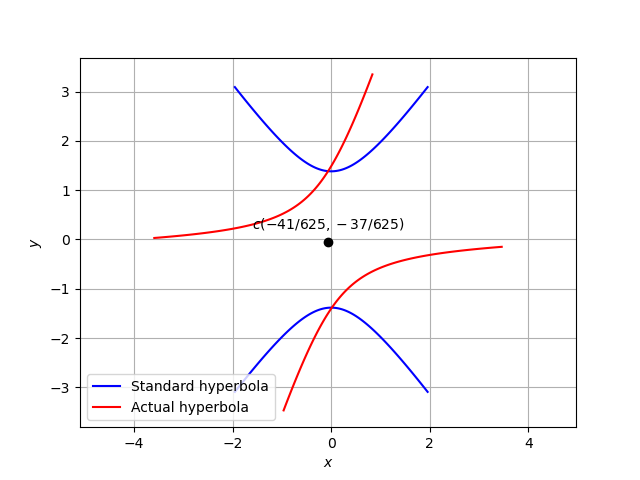
\includegraphics[width=\columnwidth]{./solutions/40/4/Hyperbola.png}
    \caption{Hyperbola when origin is shifted}
    \label{eq:solutions/40/4/Fig :1}
\end{figure}
\item  Now \eqref{eq:solutions/40/4/given} can be written as,
\begin{align}
    \vec{y}^T\vec{D}\vec{y}=\vec{u}^T\vec{V}^{-1}\vec{u}-f\label{eq:solutions/40/4/fi}
\end{align}
where ,
\begin{align}
    \vec{y}&=\vec{P}^T(\vec{x}-\vec{c})
\end{align}
To get $\vec{y}$,
\begin{align}
    \vec{y}=\vec{P}^T\vec{x}-\vec{P}^T\vec{c}\\
    \vec{y}=\myvec{\frac{-3}{4}&1\\\frac{4}{3}&1}\vec{x}-
    \myvec{\frac{-3}{4}&1\\\frac{4}{3}&1}\myvec{\frac{-41}{625}\\\frac{-37}{625}}\\
    \vec{y}=\myvec{\frac{-3}{4}&1\\\frac{4}{3}&1}\vec{x}-
    \myvec{\frac{-1}{100}\\\frac{-11}{75}}
\end{align}
Subsituting the eqauations \eqref{eq:solutions/40/4/cond}, \eqref{eq:solutions/40/4/eqDD} in equation \eqref{eq:solutions/40/4/fi}
\begin{align}
    \vec{y}^T\myvec{50&0\\0&-25}\vec{y}=\frac{-30119}{625}
\end{align}
